\documentclass[11pt]{article}
\usepackage[margin=1in]{geometry}
\usepackage{amsmath,amssymb}
\usepackage{booktabs,graphicx,caption}
\usepackage[hidelinks]{hyperref}
\setlength{\parskip}{4pt}

\title{Embodied Progress in AI versus Regular Capital:\\
Annual OLG Economy Compared with Ramsey}
\author{Research note (draft)}
\date{October 2026}

\begin{document}
\maketitle

\begin{abstract}
\noindent The embodied-progress experiments are repeated in an annual overlapping-generations economy (60 cohorts, working ages 1--45) with the same technology, shocks, adjustment costs,
depreciation and 5-year S-curve, with and without internal habits ($h=0.7$). A shock is a one-time level shift sized to raise long-run GDP by 10 percent in each model.
Over the first decade the OLG real rate is close to the Ramsey rate: the decade average differs by 0.01--0.10 points, and the AI-minus-regular gap differs by less than 0.2 points.
The two models separate afterwards. In Ramsey the long-run rate is 7.5 percent for any level shift. In the OLG economy
it is 7.5 percent for regular-capital progress but 7.61--7.62 percent for AI, because AI lowers the labor share (69.7 to 67.8 percent) and so shifts income toward capital. The AI-minus-regular gap in the real rate is
about $+0.1$ points from about year 20 in the OLG model against zero in Ramsey. The conclusion is that AI does not differ from regular capital for the real rate over the first decade in either saving model. Beyond that, AI raises the long-run rate by about 0.1 point if saving is not perfectly elastic.
\end{abstract}

\section{What changes relative to the Ramsey runs}

Everything else is as in the embodied note: Cobb-Douglas capital--labor bundle inside a CES aggregate with AI capital ($\varepsilon=1.5$), $d_A=d_K=6.6$ percent, trend growth 1.5 percent,
adjustment costs half the earlier baseline ($c_K=6.2$, $c_A=6.5$), GDP as gross value added, and the same three timings.

\paragraph{Households.} Each cohort has a lifetime of 60 years (ages 20--79), earns a flat wage for the first 45, holds wealth in a fund that owns both capital stocks, and has log utility with no bequests.
With habits the cohort maximizes $\sum_k\beta^k\ln(c_k-hc_{k-1})$. The habit stock starts at zero at entry, and cohorts alive at the time of the shock keep their own pre-shock habit stock.
The cohort Euler equation $\lambda_k=1/X_k-\beta h/X_{k+1}=\beta R\lambda_{k+1}$ (with $X=c-hc_{-1}$) is solved exactly for any path of returns: $X_k$ is proportional to the inverse of a discounted sum of future multipliers,
so a cohort's whole consumption path follows from one lifetime budget constraint. Existing cohorts' wealth is revalued by the change in the payoff to capital at date 0.

\paragraph{Calibration.} The patience parameter $\beta$ is chosen so that the initial balanced growth path has $r=7.5$ percent and the same consumption share as Ramsey ($\beta=0.939$ without habits, $0.932$ with).
The initial wealth distribution is the steady-state life-cycle profile and is consistent with the capital stock (aggregate assets equal the capital payoff to $10^{-15}$).

\paragraph{Equilibrium and long run.} Two conditions hold each year: the two capital stocks earn the same return, and consumption out of output net of investment equals the sum of cohort consumption.
Newton--Levenberg--Marquardt solves the 500 equations in the two investment-rate paths; the long-run rate comes from a one-dimensional fixed point in $r$ (closed form for the balanced growth path, as in the saving-models note).
Each shock is sized within each model for a 10 percent long-run GDP gain (regular-capital shocks are identical to Ramsey; the AI shock is 3 percent larger in logs, 1.26 against 1.22, because the long-run rate rises). With adjustment costs and habits switched off, the solver reproduces the earlier annual-OLG results to four digits.

\section{Results}

\begin{table}[h!]
\centering\small
\caption{Real rate: OLG versus Ramsey. Averages are in percentage points over 7.5 percent.}
\resizebox{\textwidth}{!}{\begin{tabular}{lllccccccc}\toprule
 & & & avg. $r$ & avg. $r$ & avg. $r$ & $r_1$ & $r$, & $r$, & long-run $r$\\
 & & & yrs 1--10 & yrs 11--20 & yrs 21--50 & & yr 20 & yr 50 & (closed form)\\
 & & & \multicolumn{3}{c}{(pp over 7.5\%)} & \multicolumn{4}{c}{(percent)}\\\midrule
S-curve & Log & Regular Ramsey & +0.26 & +0.40 & +0.10 & 7.23 & 7.75 & 7.52 & 7.50\\
 &  &  OLG & +0.20 & +0.35 & +0.08 & 7.18 & 7.71 & 7.52 & 7.50\\
 &  & AI Ramsey & +0.21 & +0.35 & +0.11 & 7.37 & 7.74 & 7.53 & 7.50\\
 &  &  OLG & +0.23 & +0.40 & +0.19 & 7.37 & 7.80 & 7.63 & 7.61\\
\addlinespace
 & Log + habits & Regular Ramsey & +0.15 & +0.39 & +0.09 & 6.64 & 7.74 & 7.52 & 7.50\\
 &  &  OLG & +0.11 & +0.33 & +0.08 & 6.71 & 7.71 & 7.52 & 7.50\\
 &  & AI Ramsey & +0.22 & +0.34 & +0.11 & 7.39 & 7.73 & 7.53 & 7.50\\
 &  &  OLG & +0.23 & +0.40 & +0.20 & 7.37 & 7.81 & 7.64 & 7.62\\
\midrule
Half/half & Log & Regular Ramsey & +0.47 & +0.35 & +0.09 & 7.84 & 7.72 & 7.52 & 7.50\\
 &  &  OLG & +0.41 & +0.29 & +0.07 & 7.78 & 7.68 & 7.52 & 7.50\\
 &  & AI Ramsey & +0.35 & +0.32 & +0.10 & 7.70 & 7.72 & 7.53 & 7.50\\
 &  &  OLG & +0.37 & +0.37 & +0.18 & 7.71 & 7.78 & 7.63 & 7.61\\
\addlinespace
 & Log + habits & Regular Ramsey & +0.59 & +0.34 & +0.08 & 8.43 & 7.71 & 7.52 & 7.50\\
 &  &  OLG & +0.52 & +0.28 & +0.07 & 8.42 & 7.68 & 7.52 & 7.50\\
 &  & AI Ramsey & +0.49 & +0.32 & +0.10 & 8.39 & 7.72 & 7.53 & 7.50\\
 &  &  OLG & +0.51 & +0.38 & +0.19 & 8.35 & 7.80 & 7.64 & 7.62\\
\midrule
Jump & Log & Regular Ramsey & +0.69 & +0.30 & +0.08 & 8.49 & 7.69 & 7.52 & 7.50\\
 &  &  OLG & +0.62 & +0.24 & +0.06 & 8.43 & 7.65 & 7.52 & 7.50\\
 &  & AI Ramsey & +0.54 & +0.28 & +0.09 & 8.21 & 7.70 & 7.53 & 7.50\\
 &  &  OLG & +0.58 & +0.34 & +0.17 & 8.24 & 7.76 & 7.63 & 7.61\\
\addlinespace
 & Log + habits & Regular Ramsey & +1.04 & +0.29 & +0.07 & 10.27 & 7.68 & 7.52 & 7.50\\
 &  &  OLG & +0.94 & +0.23 & +0.06 & 10.20 & 7.65 & 7.51 & 7.50\\
 &  & AI Ramsey & +0.87 & +0.28 & +0.09 & 9.85 & 7.69 & 7.53 & 7.50\\
 &  &  OLG & +0.89 & +0.35 & +0.18 & 9.82 & 7.78 & 7.64 & 7.62\\
\midrule
\bottomrule\end{tabular}
}
\end{table}

\begin{figure}[h!]
\centering
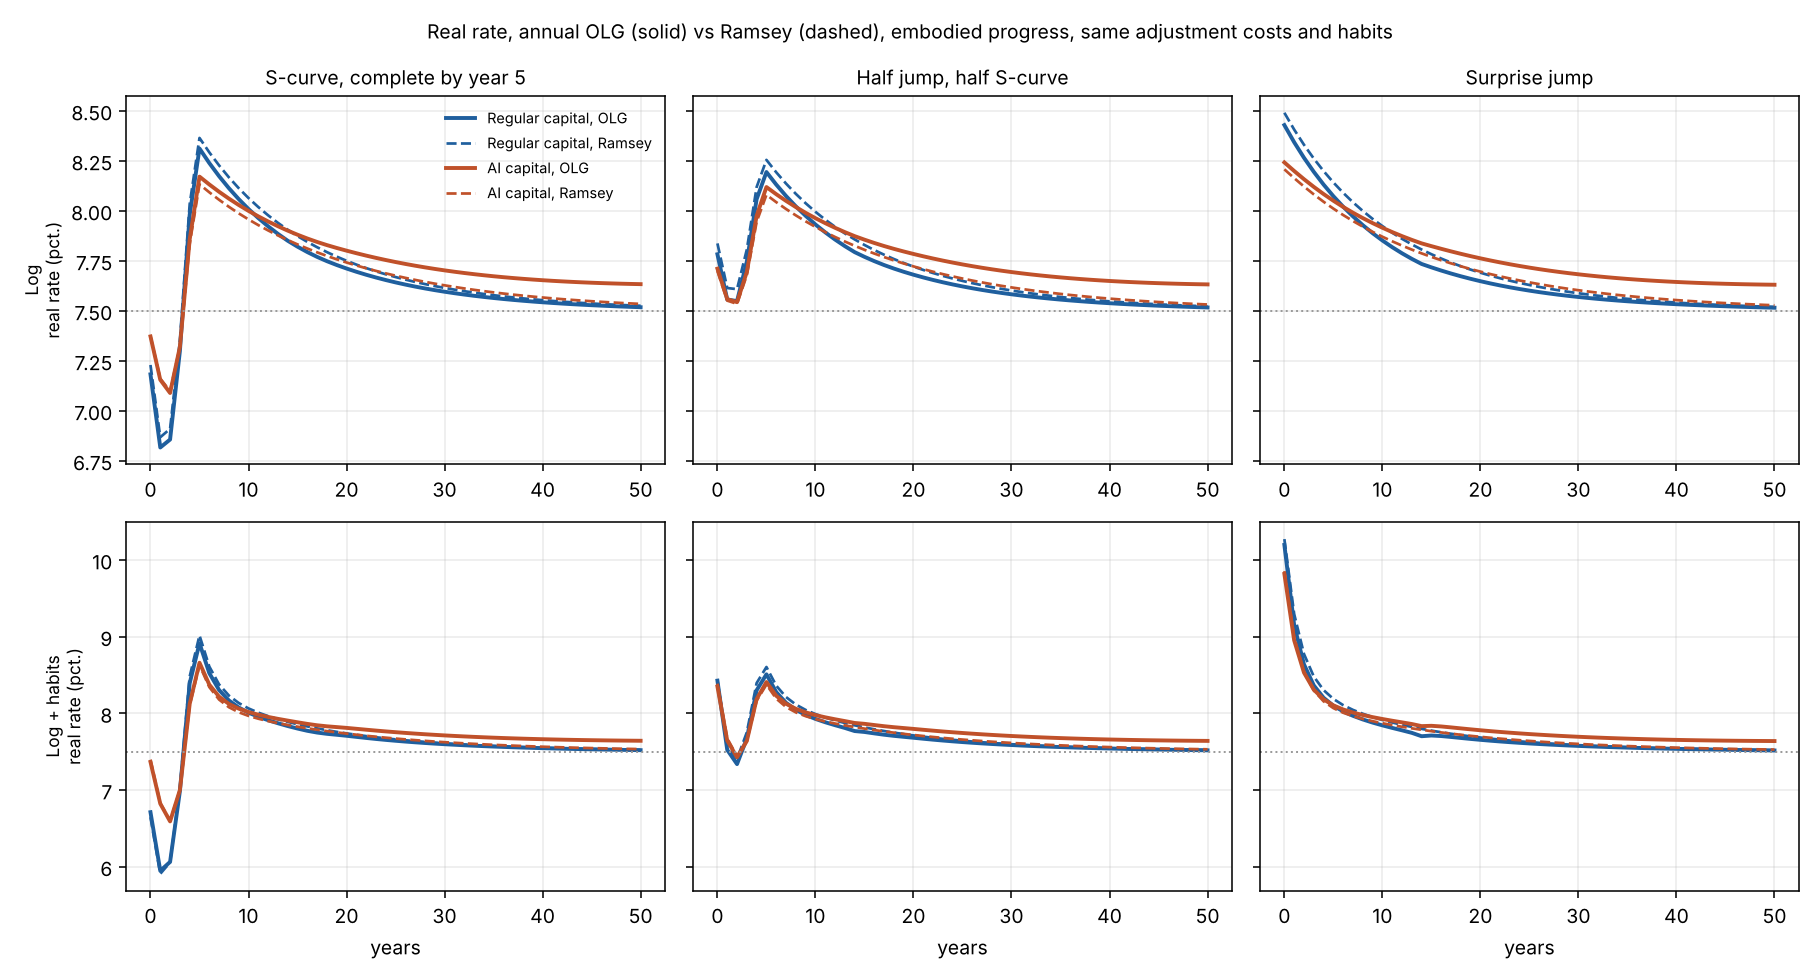
\includegraphics[width=\textwidth]{figures/fig_olg_r.png}
\caption{Real rate, OLG (solid) versus Ramsey (dashed).}
\end{figure}

\paragraph{First decade.} The OLG and Ramsey rates are close. With log utility, the decade average after regular-capital progress is $+0.20$ (OLG) against $+0.26$ (Ramsey) for the S-curve and $+0.62$ against $+0.69$ for the jump.
With habits the figures are $+0.11$ against $+0.15$ and $+0.94$ against $+1.04$. For AI the two models differ by 0.01--0.04 points. Habits matter more than the saving model for the jump: they raise the impact rate from 8.4 to 10.2 percent (OLG, regular) and from 8.2 to 9.8 percent (AI).
Life-cycle saving is slightly less responsive than the representative household's, so the impact rate is a little lower in the OLG model.

\paragraph{AI versus regular capital.} Table~\ref{tab:gap} gives the gap.

\begin{table}[h!]
\centering\small
\caption{AI minus regular capital, average real rate in percentage points.}\label{tab:gap}
\begin{tabular}{llcccccc}\toprule
 & & \multicolumn{3}{c}{AI $-$ regular, OLG (pp)} & \multicolumn{3}{c}{AI $-$ regular, Ramsey (pp)}\\
 & & yrs 1--10 & yrs 11--20 & yrs 21--50 & yrs 1--10 & yrs 11--20 & yrs 21--50\\\midrule
S-curve & Log & +0.03 & +0.05 & +0.11 & -0.05 & -0.05 & +0.01\\
 & Log + habits & +0.13 & +0.07 & +0.12 & +0.07 & -0.04 & +0.01\\
\midrule
Half/half & Log & -0.03 & +0.08 & +0.11 & -0.12 & -0.03 & +0.01\\
 & Log + habits & -0.01 & +0.09 & +0.12 & -0.10 & -0.02 & +0.01\\
\midrule
Jump & Log & -0.05 & +0.10 & +0.11 & -0.15 & -0.02 & +0.01\\
 & Log + habits & -0.06 & +0.12 & +0.12 & -0.17 & -0.01 & +0.01\\
\bottomrule\end{tabular}

\end{table}

\begin{figure}[h!]
\centering
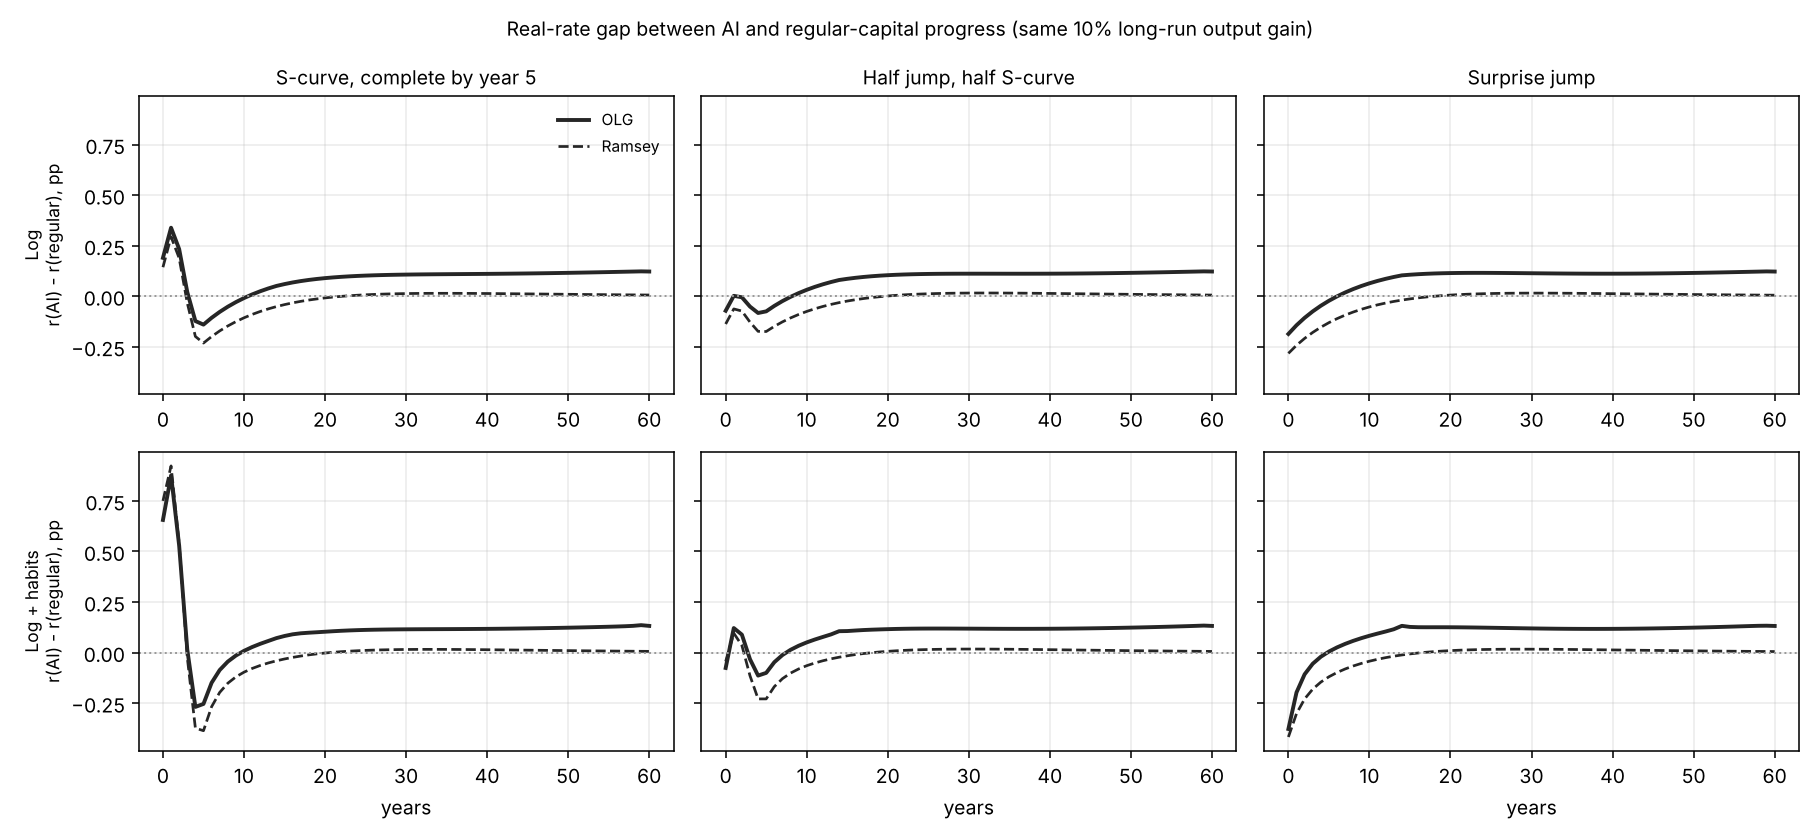
\includegraphics[width=\textwidth]{figures/fig_olg_gap.png}
\caption{Real-rate gap between AI and regular-capital progress.}
\end{figure}

In the first decade the OLG gap is between $-0.06$ and $+0.13$ points and the Ramsey gap between $-0.17$ and $+0.07$, so neither is distinguishable from zero in economic terms, and its sign depends on timing and habits.
In years 11--20 the OLG gap is $+0.05$ to $+0.12$ points and in years 21--50 it settles at $+0.11$ to $+0.12$, while in Ramsey it is between $-0.05$ and $0$ and then $+0.01$. The long-run rates are 7.50 percent (regular) and 7.61--7.62 percent (AI) in the OLG model.
The long-run difference comes from the capital share rising by 1.9 points with AI and not with regular capital: the fixed-point condition for the OLG economy then requires a slightly higher return to equate the wealth that households want to hold with the wealth the economy needs.
The effect is small because the AI share starts at 3 percent; this note does not separately identify how elastic life-cycle saving is.

\paragraph{Real variables.} The real side is almost the same in the two models, so the earlier findings on output and investment carry over (Table~\ref{tab:real}).

\begin{table}[h!]
\centering\small
\caption{GDP, investment share, wage and labor share, OLG versus Ramsey.}\label{tab:real}
\resizebox{\textwidth}{!}{\begin{tabular}{llcccccc}\toprule
 & & GDP gap closed, yr 10 (\%) & $\Delta$ inv./GDP yr 10 (pp) & $\Delta$ inv./GDP yr 20 (pp) & $\ln W$, yr 10 (\%) & labor share yr 10 (\%) & labor share, long run (\%)\\\midrule
S-curve & Log Regular Ramsey & 0 & +0.76 & +0.34 & 4.1 & 69.7 & 69.6\\
 &  Regular OLG & 0 & +0.84 & +0.37 & 4.2 & 69.7 & 69.6\\
 &  AI Ramsey & 0 & +1.38 & +1.26 & 2.4 & 68.8 & 67.8\\
 &  AI OLG & 0 & +1.36 & +1.20 & 2.5 & 68.8 & 67.8\\
\midrule
 & Log + habits Regular Ramsey & 0 & +0.80 & +0.36 & 4.1 & 69.7 & 69.6\\
 &  Regular OLG & 0 & +0.87 & +0.37 & 4.2 & 69.7 & 69.6\\
 &  AI Ramsey & 0 & +1.40 & +1.27 & 2.3 & 68.8 & 67.8\\
 &  AI OLG & 0 & +1.37 & +1.19 & 2.4 & 68.8 & 67.8\\
\midrule
Half/half & Log Regular Ramsey & 0 & +0.67 & +0.30 & 4.8 & 69.7 & 69.6\\
 &  Regular OLG & 0 & +0.75 & +0.33 & 4.9 & 69.7 & 69.6\\
 &  AI Ramsey & 0 & +1.36 & +1.24 & 2.8 & 68.7 & 67.8\\
 &  AI OLG & 0 & +1.34 & +1.18 & 2.8 & 68.7 & 67.8\\
\midrule
 & Log + habits Regular Ramsey & 0 & +0.71 & +0.32 & 4.8 & 69.7 & 69.6\\
 &  Regular OLG & 0 & +0.79 & +0.33 & 4.9 & 69.7 & 69.6\\
 &  AI Ramsey & 0 & +1.39 & +1.26 & 2.7 & 68.7 & 67.8\\
 &  AI OLG & 0 & +1.35 & +1.17 & 2.8 & 68.7 & 67.8\\
\midrule
Jump & Log Regular Ramsey & 1 & +0.58 & +0.26 & 5.6 & 69.7 & 69.6\\
 &  Regular OLG & 1 & +0.67 & +0.29 & 5.7 & 69.7 & 69.6\\
 &  AI Ramsey & 0 & +1.34 & +1.22 & 3.3 & 68.6 & 67.8\\
 &  AI OLG & 0 & +1.31 & +1.15 & 3.4 & 68.5 & 67.8\\
\midrule
 & Log + habits Regular Ramsey & 1 & +0.62 & +0.28 & 5.5 & 69.7 & 69.6\\
 &  Regular OLG & 1 & +0.70 & +0.28 & 5.6 & 69.7 & 69.6\\
 &  AI Ramsey & 0 & +1.37 & +1.24 & 3.2 & 68.6 & 67.8\\
 &  AI OLG & 0 & +1.32 & +1.15 & 3.3 & 68.5 & 67.8\\
\bottomrule\end{tabular}
}
\end{table}

\section{Caveats}
\begin{itemize}
\item Habit formation at the cohort level is a modeling choice: the zero habit stock at entry is arbitrary. It affects mainly the shape of the age profile, not the aggregate response, because the shock is announced to all cohorts.
\item The OLG long-run rate is a small effect (about 0.1 point) and depends on the calibration of the age profile and on the initial AI share of 3 percent. A larger initial AI share, or $\varepsilon=2$, would give a larger difference, as in the elasticity grid of the saving-models note.
\item Depreciation, adjustment costs and shock sizes are those of the embodied note; none was changed here.
\item The model has fixed hours and flexible prices. Interest-rate effects of nominal rigidities are not included.
\end{itemize}

\section*{Appendix: numerical checks}
\begin{table}[h!]
\centering\small
\begin{tabular}{lc}\toprule Check & max abs. error\\\midrule
OLG residual & 8.8e-10\\
Ramsey residual & 2.7e-12\\
OLG long-run ln Y = 10\% & 2.7e-06\\
initial BGP solves the OLG equilibrium & 3.3e-15\\
\bottomrule\end{tabular}

\end{table}
\end{document}
